\documentclass[10pt]{beamer}

\usepackage[utf8]{inputenc}
\usepackage[english]{babel}
\setbeamersize{text margin left=5mm,text margin right=5mm} 

\usepackage{amssymb,amsmath,amsthm,amsfonts,mathtools}

\mathtoolsset{showonlyrefs}

\let\caron\v %caron accent %https://en.wikibooks.org/wiki/LaTeX/Special_Characters#Escaped_codes

\renewcommand{\a}{\alpha}
\renewcommand{\b}{\beta}
\renewcommand{\c}{\chi}
\renewcommand{\d}{\delta}
\newcommand{\e}{\epsilon}
\newcommand{\f}{\phi}
\newcommand{\g}{\gamma}
\newcommand{\h}{\hbar}
\renewcommand{\i}{\iota}
\renewcommand{\j}{\varepsilon}
\renewcommand{\k}{\kappa}
\renewcommand{\l}{\lambda}
\newcommand{\m}{\mu}
\newcommand{\n}{\nu}
\renewcommand{\o}{\omega}
\newcommand{\p}{\psi}
\newcommand{\q}{\eta}
\renewcommand{\r}{\rho}
\newcommand{\s}{\sigma}
\renewcommand{\t}{\theta}
\renewcommand{\u}{\pi}
\renewcommand{\v}{\varphi}
\newcommand{\w}{\tau}
\newcommand{\x}{\xi}
\newcommand{\y}{\upsilon}
\newcommand{\z}{\zeta}

\newcommand{\A}{\nabla}
\newcommand{\B}[1]{\Big#1}
\newcommand{\C}{\mathbb C}
\newcommand{\D}{\Delta}
\newcommand{\E}{\mathbb E}
\newcommand{\F}{\Phi}
\newcommand{\G}{\Gamma}
\renewcommand{\H}{\mathbb H}
\newcommand{\I}[1]{\tensor[]{}{#1}}
\renewcommand{\L}{\Lambda}
\newcommand{\N}{\mathbb N}
\renewcommand{\O}{\Omega}
\renewcommand{\P}{\Psi}
\newcommand{\R}{\mathbb R}
\renewcommand{\S}{\Sigma}
\newcommand{\T}{\Theta}
\newcommand{\U}{\Pi}
\newcommand{\V}{\wedge}
\newcommand{\X}{\Xi}
\newcommand{\Y}{\mathbb Y}
\newcommand{\Z}{\mathbb Z}

\newcommand{\cA}{\mathcal A}
\newcommand{\cD}{\mathcal D}
\newcommand{\cF}{\mathcal F}
\newcommand{\cG}{\mathcal G}
\newcommand{\cI}{\mathcal I}
\newcommand{\cL}{\mathcal L}
\newcommand{\cM}{\mathcal M}
\newcommand{\cN}{\mathcal N}
\newcommand{\cO}{\mathcal O}
\newcommand{\cS}{\mathcal S}
\newcommand{\cT}{\mathcal T}
\newcommand{\cZ}{\mathcal Z}

\newcommand{\fF}{\mathfrak F}
\newcommand{\fg}{\mathfrak g}
\newcommand{\fh}{\mathfrak h}
\newcommand{\fk}{\mathfrak k}
\newcommand{\fm}{\mathfrak m}
\newcommand{\fn}{\mathfrak n}

\newcommand{\dd}{\mathrm{d}}
\newcommand{\ha}[1]{\hat #1}
\newcommand{\la}{\langle}
\newcommand{\ra}{\rangle}
\newcommand{\ti}[1]{\tilde #1}
\newcommand{\bs}[1]{\boldsymbol #1}
\newcommand{\pd}{\partial}
\newcommand{\at}[1]{\vert_{#1}}
\newcommand{\At}[1]{\B\vert_{#1}}
\newcommand{\der}[2]{\frac{\dd#1}{\dd#2}}
\newcommand{\pder}[2]{\frac{\partial#1}{\partial#2}}
\newcommand{\derat}[3]{\der{#1}{#2}\at{#3}}
\newcommand{\pderat}[3]{\pder{#1}{#2}\At{#3}}
\newcommand{\fder}[2]{\frac{\d#1}{\d#2}}
\newcommand{\fderat}[3]{\fder{#1}{#2}\At{#3}}
\newcommand{\id}{\textrm{id}}
\newcommand{\into}{\hookrightarrow}
\newcommand{\onto}{\twoheadrightarrow}
\newcommand{\dmap}{\overset\dd\longrightarrow}
\newcommand{\inv}[1]{#1^{-1}}
\newcommand{\defeq}{:=}


\newcommand{\ham}{hamiltonian}
\newcommand{\lag}{lagrangian}
\newcommand{\eom}{equation of motion}
\newcommand{\eoms}{equations of motion}
\newcommand{\dof}{degree of freedom}
\newcommand{\dofs}{degrees of freedom}
\newcommand{\off}{off-shell}
\newcommand{\on}{on-shell}
\newcommand{\vf}{vector field}
\newcommand{\vfs}{vector fields}
\newcommand{\wrt}{with respect to\ }
\newcommand{\nbh}{neighbourhood}
\newcommand{\ex}{exterior differential}
\newcommand{\ie}{i.e.\@\ }
\newcommand{\eg}{e.g.\@\ }
\newcommand{\st}{s.t.\@\ }
\newcommand{\susy}{supersymmetry}
\newcommand{\sugra}{supergravity}
\newcommand{\rhs}{r.h.s.\@\ }
\newcommand{\lhs}{l.h.s.\@\ }
\newcommand{\rs}{Riemann surface}
\newcommand{\rss}{Riemann surfaces}
\newcommand{\hn}{Hurwitz number}
\newcommand{\hnn}{Hurwitz numbers}
\newcommand{\cpt}{compact}
\newcommand{\cpx}{complex}
\newcommand{\const}{constant}
\newcommand{\holo}{holomorphic}
\newcommand{\branch}{\textsc{Branch}}
\newcommand{\tiff}{if and only if\ }

\newcommand{\YM}{Yang-Mills}
\newcommand{\sYM}{super Yang-Mills}
\newcommand{\SYM}{Super-Yang-Mills}

\renewcommand{\det}{\operatorname{det}}
\newcommand{\End}{\operatorname{End}}
\newcommand{\Lie}{\operatorname{Lie}}
\newcommand{\Map}{\operatorname{Map}}
\newcommand{\Ber}{\operatorname{Ber}}
\newcommand{\diag}{\operatorname{diag}}
\newcommand{\tr}{\operatorname{tr}}
\newcommand{\Vol}{\operatorname{Vol}}
\newcommand{\im}{\operatorname{im}}
\newcommand{\Aut}{\operatorname{Aut}}


\newcommand{\tand}{\quad\text{and}\quad}
\newcommand{\tcomma}{\ ,\qquad}
\newcommand{\tfor}{\quad\text{for}\quad}
\newcommand{\tforall}{\quad\text{for all}\quad}
\newcommand{\imply}{\quad\Rightarrow\quad}
\newcommand{\implied}{\quad\Leftarrow\quad}
\renewcommand{\iff}{\quad\Leftrightarrow\quad}
\newcommand{\twith}{\quad\text{with}\quad}
\newcommand{\twhere}{\quad\text{where}\quad}
\newcommand{\tif}{\quad\text{if}\ }

\newcommand{\tleft}{\text{left}}
\newcommand{\tright}{\text{right}}
\newcommand{\ttop}{\text{top}}
\newcommand{\tint}{\text{int}}
\newcommand{\tst}{\text{st}}
\newcommand{\tss}{\text{ss}}
\newcommand{\tps}{\text{ps}}
\newcommand{\tgm}{\text{gm}}
\newcommand{\tsugra}{\text{sugra}}
\newcommand{\trigid}{\text{rigid}}
\newcommand{\tclosed}{\text{closed}}
\newcommand{\texact}{\text{exact}}
\newcommand{\tCS}{\text{CS}}
\newcommand{\tclass}{\text{class}}

\newcommand{\cclass}{\C_\tclass}

\newcommand{\Rnm}{\R^{n|m}}


\usetheme{Warsaw}
\usecolortheme{default}
\usefonttheme{professionalfonts}

%gets rid of bottom navigation bars
\setbeamertemplate{footline}[frame number]{}

%gets rid of bottom navigation symbols
%\setbeamertemplate{navigation symbols}{}

%gets rid of footer
%will override 'frame number' instruction above
%comment out to revert to previous/default definitions
\setbeamertemplate{footline}{}

%environment for equations
\usepackage{xparse}
\NewDocumentCommand \deq { o m }{
  \setlength\abovedisplayskip{4pt}
  \setlength\belowdisplayskip{4pt}
  \setlength\abovedisplayshortskip{0pt}
  \setlength\belowdisplayshortskip{3pt}
\begin{equation}
\begin{aligned}
{}#2
\IfNoValueF{#1}{\label{#1}}
\end{aligned}
\end{equation}
}


\usepackage[backend=biber, style=verbose, sorting=ynt]{biblatex}
\addbibresource{../biblio-beamer.bib}
\setbeamertemplate{bibliography item}{\insertbiblabel}

%------------------------------------------------------------
%This block of code defines the information to appear in the
%Title page
\title[Hurwitz numbers in half infinite wedge space] %optional
{Hurwitz numbers in half infinite wedge space}

\subtitle{From geometry to operators}

\author[Arthur, Doe] % (optional)
{Andrea Grossutti}

\institute[VFU] % (optional)
{SISSA
  %\inst{1}%
  %Faculty of Physics\\
  %Very Famous University
  %\and
  %\inst{2}%
  %Faculty of Chemistry\\
  %Very Famous University
}

\date[VLC 2021] % (optional)
{%Very Large Conference, 
	May 2021}

%End of title page configuration block
%------------------------------------------------------------



%------------------------------------------------------------
%The next block of commands puts the table of contents at the 
%beginning of each section and highlights the current section:

\AtBeginSubsection[]
{
  \begin{frame}
    \frametitle{Table of Contents}
    \tableofcontents[currentsection,currentsubsection]
  \end{frame}
}
%------------------------------------------------------------

\begin{document}

%The next statement creates the title page.
\frame{\titlepage}


%---------------------------------------------------------
%This block of code is for the table of contents after
%the title page
\begin{frame}
\frametitle{Table of Contents}
\tableofcontents
\end{frame}
%---------------------------------------------------------

\section{From Hurwitz numbers to Burnside's formula}
\subsection{Maps of \rss\ and \hnn}

\begin{frame}

Let $f\colon X\to Y$ be a (non-\const\ \holo) map of (\cpt) and connected \rss\ (hence surjective).

\begin{definition}
	\begin{itemize}
		\item The \emph{ramification index} of $f$ at $x\in X$ is the integer $k_x\in\Z_{\geq1}$ \st $f$ is locally of the form $z^k$, where $z$ is a local coordinate centered in $x$. 
		\item The \emph{differential length} of $f$ at $x\in X$ is $\nu_x=k_x-1$.
		\item A point $x\in X$ \st $\nu_x>0$ is called a \emph{ramification point}. The \emph{ramification locus} of $f$ is the set of its ramification points. If $\n_x=0$ we say that $f$ is \emph{unramified} at $x$. If $\n_x=1$ we say that $f$ has \emph{simple ramification} at $x$. 
		\item If $x\in X$ is a ramification point, then $f(x)\in Y$ is called a \emph{branch point}. The \emph{branch locus} $B_f$ of $f$ is the set of its branch points.
	\end{itemize}
\end{definition}

For any $y,y'\in Y\setminus B_f$ we have $|\inv f(y)|=|\inv f(y')|$. 

\begin{definition}
	\vspace{-5pt}
	\deq{\deg f\defeq|\inv f(y)|\tcomma y\in Y\setminus B_f\ .}
\end{definition}

\end{frame}

%--------------------------------------------------------

\begin{frame}

For any $y\in Y$, $\inv f(y)=\{x_1,\ldots,x_n\}$, we have $d:=\deg f=\sum_ik_{x_i}$.

\begin{definition}
	We call \emph{ramification profile} of $f$ at $y$ the partition of $d$ given by $(k_{x_1},\ldots,k_{x_n})$. We say that $f$ is \emph{unramified} / \emph{simply ramified} / \emph{fully ramified} if its ramification profile is $(1,\ldots,1)$ / $(2,1,\ldots,1)$ / $(d)$ respectively.
\end{definition}

\begin{theorem}[Riemann-Hurwitz]
	Let $g_X$ and $g_Y$ denote the genus of $X$ and $Y$ respectively. Then
	\deq{\underbrace{2g_X-2}_{\c(X)}=(\underbrace{2g_Y-2}_{\c(Y)})\deg f+\sum_{x\in X}\nu_x}
\end{theorem}

\begin{definition}
	$f\colon X\to Y$ and $g\colon\ti X\to Y$ are \emph{isomorphic} if there is $\f\colon X\overset\sim\to\ti X$ \st $f=g\circ \f$. 
	
	An \emph{automorphism} of $f\colon X\to Y$ is $\p\colon X\overset\sim\to X$ \st $f=f\circ \p$. \\The group of automorphisms of $f$ is denoted $\Aut(f)$. 

\end{definition}

\end{frame}

%--------------------------------------------------------



\begin{frame}

\begin{definition}
	Let $Y$ RS of genus $g$, $B=\{b_1,\ldots,b_n\}\subset Y$, $d\geq0$, $\q_1,\ldots,\q_n\prt d$. \\We define the \emph{(degree $d$) connected Hurwitz number} to be 
	\deq{H^\circ_{h\overset d\to g}(\q_1,\ldots,\q_n):=\sum_{[f]}\frac1{|\Aut(f)|}}
	and the \emph{(disconnected) (degree $d$) Hurwitz number} to be
	\deq{H^\bullet_{h\overset d\to g}(\q_1,\ldots,\q_n):=\sum_{[f]}\frac1{|\Aut(f)|} \label{eq:disc-H-numb}}
	where both sums runs over isomorphism classes of degree $d$ \holo\ maps $f\colon X\to Y$ \st
	\begin{itemize}
		\item $X$ is a \cpt\ RS of genus $h$
		\item the branch locus of $f$ is $B$
		\item the ramification profile of $f$ at $b_i$ is $\q_i$
	\end{itemize}
	In the case of connected Hurwitz numbers we further require $X$ to be connected.
\end{definition}

\end{frame}

%--------------------------------------------------------

\subsection{Maps of \rss\ as ramified covers}

\begin{frame}

Maps of \rss\ are ramified covers:

\begin{definition}
	A \emph{ramified cover} is a continuous function between compact topological surfaces $f\colon X\to Y$ with a finite set $B\subset Y$ \st
	\begin{itemize}
		\item$\inv f(B)$ is finite,
		\item $f\colon X\setminus\inv f(B)\to Y\setminus B$ is a covering.
	\end{itemize}
\end{definition}

Vice-versa, we have

\begin{theorem}[Riemann's Existence Thm.] 
	Let $Y$ \cpt\ \rs, $X^0$ topological surface, $\{b_1,\ldots,b_n\}\subset Y$ finite subset, $f^0\colon X^0\to Y\setminus\{b_1,\ldots,b_n\}$ covering of finite degree. Then there exists a unique (up to isomorphisms) \cpt\ \rs\ $X$ \st
	\begin{itemize}
		\item $X^0$ is a dense subset of $X$,
		\item $f^0$ extends to a \holo\ map of \rss\ $f\colon X\to Y$.
	\end{itemize}
\end{theorem}

This will be useful to reconstruct $X$ and $f$ given $Y$ and some additional data.

\end{frame}

%---------------------------------------------------------

\begin{frame}

\begin{definition}
	The map $f\colon X\to Y$ is said \emph{$y_0$-labelled} if $y_0\in Y\setminus B_f$ and is chosen an isomorphism $L\colon \inv f(y_0)\overset\sim\to \{1,\ldots,d\}$. We also say that $L$ is a \emph{labelling}. An \emph{isomorphism of $y_0$-labelled maps} $(f,L)$ and $(f',L')$ is an isomorphism of \rss\ $\f\colon X\to X'$ \st 
	\deq{f'\circ\f=f\tand L'\circ\f=L}
\end{definition}

\begin{definition}
	A $y_0$-labelled map $f\colon X\to Y$ determines a group homomorphism 
	\deq{
		\F\colon\u_1(Y\setminus B_f,y_0)\to S_d\tcomma \g\mapsto\s_\g
	}
	called \emph{monodromy representation}.
\end{definition}

We have that $(f,L)\cong(f',L')$ imply $\F=\F'$.

\end{frame}

%---------------------------------------------------------

\begin{frame}

Now consider $b\in B_f$ and $\g\in\u_1(Y\setminus B_f,y_0)$ simple loop winding once around $b$ (and with zero winding number around the other branch points). If the ramification profile of $f$ at $b$ is $\q=(k_1,\ldots,k_l)$, then $\s_\g$ has cycle type $\q$ (to see this recall that the local expression of $f$ around ramification points is $z^k$ and consider a circle around $y_0$ of unit radius in the chart).

\begin{definition}
	Let $Y$ be a connected \rs\ of genus $g$, $y_0,b_1,\ldots,b_n\in Y$ points, $d\in\Z_{\geq1}$ and $\q_1,\ldots,\q_n\prt d$. A \emph{monodromy representation of type} $(g,d,\q_1,\ldots,\q_n)$ is a group homomorphism $\F\colon\u_1(Y\setminus\{b_1,\ldots,b_n\},y_0)\to S_d$ \st if $\g_k$ is a small loop around $b_k$ then $\F(\g_k)$ has cycle type $\q_k$.
	
	If moreover the subgroup $\im \F\subset S_d$ acts transitively on $\{1,2,\ldots,d\}$ we say that $\F$ is a \emph{connected monodromy representation of type} $(g,d,\q_1,\ldots,\q_n)$.
	
\end{definition}

Note that if two labellings $L,L'$ of $f\colon X\to Y$ are given, then $L'=\s\cdot L$ for some $\s\in S_d$ and $\F'(\g)=\s\cdot\F(\g)\cdot\inv\s$. In particular the type of the monodromy representation does note depend on the chosen labelling. 

\end{frame}

\begin{frame}

We obtained that a degree $d$ map $f\colon X\to Y$ between \cpt\ connected \rss\ \st the ramification profile over each branch point is $\q_i$ gives rise to a connected monodromy representation $\F$ of type $(g_Y,d,\q_1,\ldots,\q_n)$. If we let $X$ to be non connected, then the monodromy representation may not be connected anymore, more precisely: the monodromy representation is connected \tiff $X$ is connected. We also have that isomorphic maps give the same monodromy representation. 

Conversely:

\begin{theorem}
	Let $Y$ be a \rs\ of genus $g$, $\F$ a monodromy representation of type $(g,d,\q_1,\ldots,\q_n)$, $B=\{b_1,\ldots,b_n\}\subset Y$ a finite subset. Then exists a $y_0$-labelled \holo\ map of \rs\ covering $Y$ with branch locus $B$ whose associated monodromy is $F$. Such map is unique up to isomorphisms of $y_0$-labelled maps. 
\end{theorem}

\end{frame}

\begin{frame}

\emph{\bf Sketch of proof}
	In the proof of this result the Riemann's Existence theorem is fundamental. We construct explicitly the topological space $X_0$ and the covering $f^0\colon X^0\to Y\setminus B$ in such a way that the map $f\colon X\to Y$ given by the Riemann's Existence theorem has the desired monodomy representation. 
	
	Take cycles $\a_1,\ldots\a_g,\b_1,\ldots,\b_g$ in $Y$ generating $\pi_1(Y,y_0)$ all containing a point $p\in Y$ in such a way that $Y\setminus\{\a_1,\ldots\a_g,\b_1,\ldots,\b_g\}$ is the fundamental polygon describing $Y$. Denote by $\g_i$ a loop containing $y_0$, winding once around $b_i$, never around the other elements of $B$, and fully contained in $Y\setminus\{\a_1,\ldots\a_g,\b_1,\ldots,\b_g\}$.
	
	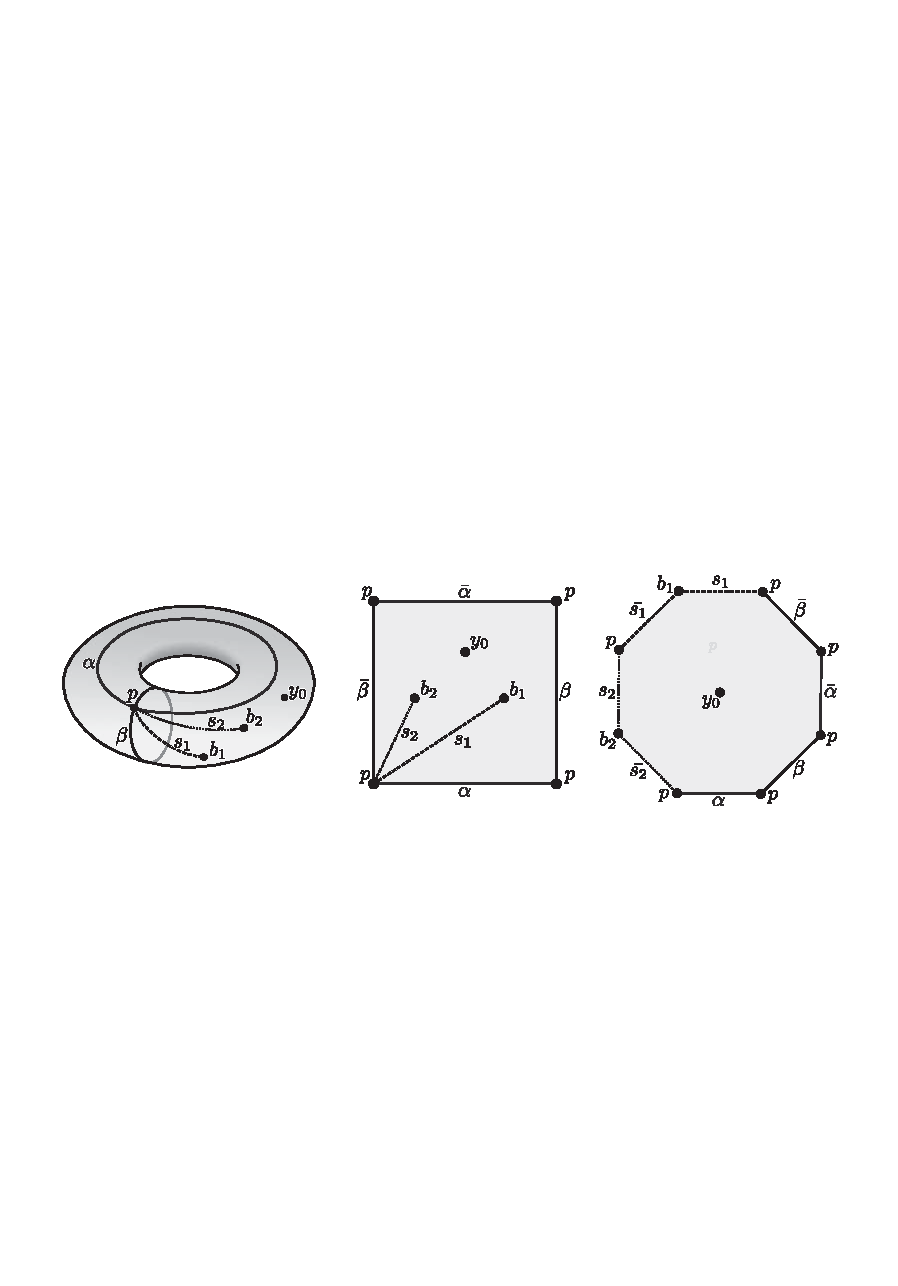
\includegraphics[width=\textwidth]{../figures/CM-fig-7-6.pdf}
	
\end{frame}

\begin{frame}
	\vspace{-10pt}
	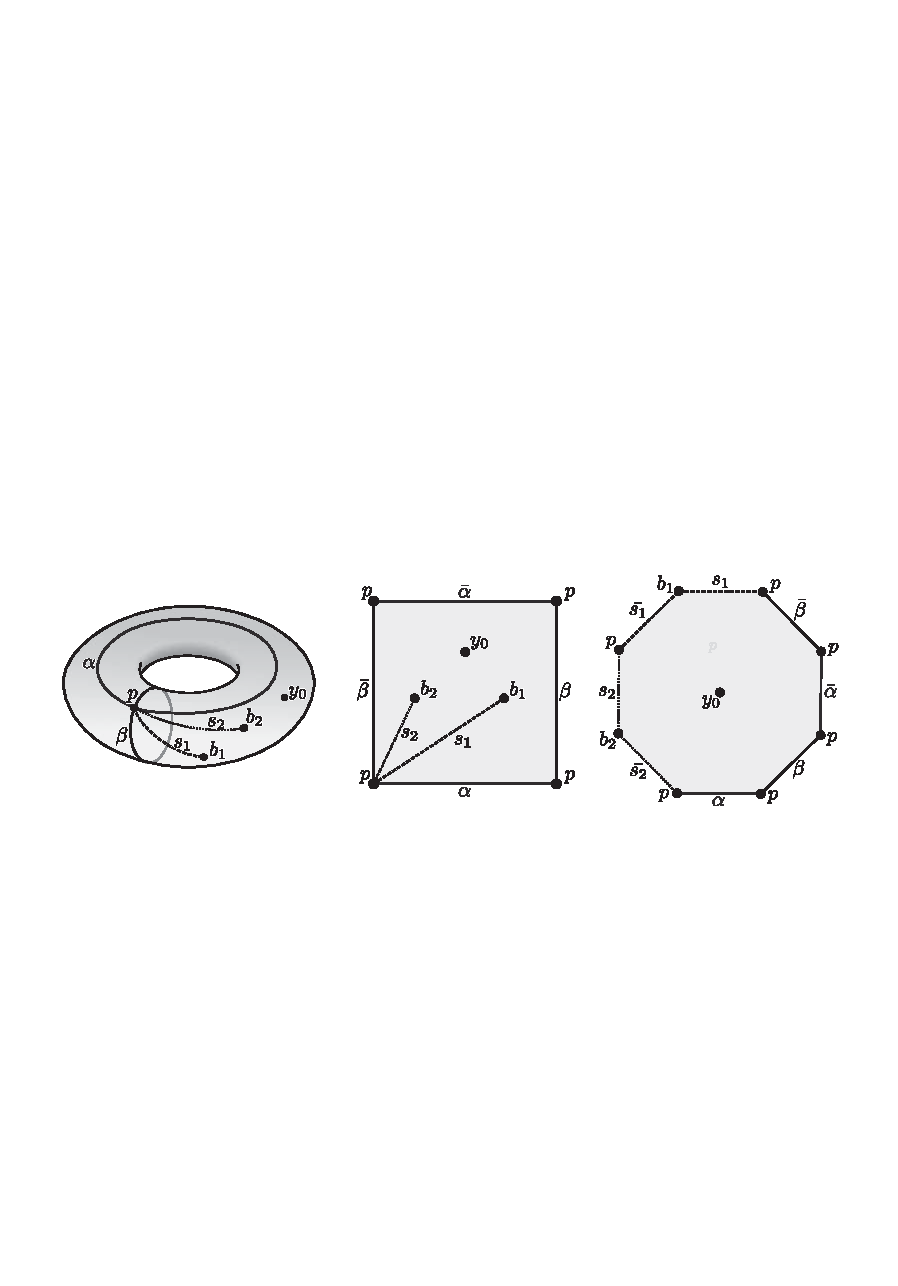
\includegraphics[width=0.9\textwidth]{../figures/CM-fig-7-6.pdf}
	
	Consider segments $s_j$ connecting $p$ with the points $b_j$. Open the previous polygon in correspondence of these segments, so that we get a new polygon
	\deq{P:=s_1\ba{s}_1\cdots s_n\ba{s}_n\a_1\b_1\ba{\a}_1\ba{\b}_1\cdots\a_g\b_g\ba{\a}_g\ba{\b}_g}
	Then it suffices to take $d$ copies of $P$ and glue their boundaries appropriately to produce $X^0$ in such a way that the natural projection to $Y\setminus B$ has the desired monodromy representation:\\[-10pt]
	\deq{s_{j,k}&\sim\ba s_{j,\F(\g_j)(k)}\\
		\ba\a_{i,k}&\sim \a_{i,\F(\b_i)(k)}\\
		\b_{i,k}&\sim \ba\b_{i,\F(\a_i)(k)}}\\[-10pt]
	
	\hfill$\blacksquare$
\end{frame}

\begin{frame}

The previous theorem ensures that we have a bijection between isomorphism classes of $y_0$-labeled Hurwitz covers and connected monodromy representations of type $(g,d,\q_1,\ldots,\q_n)$. Then we can prove

\begin{theorem}
	Let $M^\circ$ (resp $M^\bullet$) be the set of connected monodromy representations (resp. monodromy representations) of type $(g,d,\q_1,\ldots,\q_n)$. Then
	\deq{H^\circ_{h\overset d\to g}(\q_1,\ldots,\q_n)=\frac{|M^\circ|}{d!}}
	and
	\deq{H^\bullet_{h\overset d\to g}(\q_1,\ldots,\q_n)=\frac{|M^\bullet|}{d!}}
	where $h$ is determined by Riemann-Hurwitz. 
\end{theorem}

\emph{\bf Sketch of proof}
	We give the proof in the connected case, the other case is analogous. 

\end{frame}

\begin{frame}


	
	Take $f\colon X\to Y$ Hurwitz cover. Clearly there are $d!$ possible choices of a $y_0$-labelling $L\colon \inv f(y_0)\to \{1,\ldots,d\}$. An automorphism $\f\in\Aut(f)$ is an isomorphism $\f\colon X\overset\sim\to X$ satisfying $f=f\circ\f$. In particular $\f$ gives an isomorphism $(f,L)\cong(f,L')$ where $L'=\f\cdot L:=L\circ\inv\f$. Here $\f\cdot L$ denotes the left action of $\Aut(f)$ on the possible $y_0$-labellings of $f$. Such action is free (\ie $\f\cdot L=L$ imply $\f=\id_X$) so the number of isomorphism classes of $y_0$-labelings of $f$ is $d!/|\Aut(f)|$. 
	
	From the previous theorem isomorphism classes of $y_0$-labelled maps for the given $f$ are in bijection with the distinct monodromy representations arising from $f$ by different labelings of $\inv f(y_0)$. Therefore 
	\deq{m_f=\frac{d!}{|\Aut(f)|}}
	where $m_f$ the number of distinct monodromy representations arising from $f$ by different labelings of $\inv f(y_0)$. So we have
	\deq{H^\circ_{h\overset d\to g}(\q_1,\ldots,\q_n):=\sum_{[f]}\frac1{|\Aut(f)|}=\sum_{[f]}\frac{m_f}{d!}=\frac{|M^\circ|}{d!}}\\[-5mm]
	\hfill$\blacksquare$
\end{frame}

\begin{frame}

Although the information carried by connected Hurwitz numbers is usually more interesting for geometrical purposes, it turns out that it is easier to compute the (possibly disconnected) Hurwitz numbers. We will see later how it is possible to recover the connected Hurwitz numbers from the disconnected ones. 

We mention that using some ``degeneration formulas'' (which heuristically correspond to shrink the \rs\ Y producing nodal curves) all disconnected degree $d$ Hurwitz numbers are determined in therms of Hurwitz numbers of the form $H^\bullet_{h\overset d\to0}(\q_1,\q_2,\q_3)$. For this reason (and others) we later restrict our discussion to the case $g=0$. 



Using the last theorem the problem of computing degree $d$ Hurwitz numbers can be translated into a problem in representation theory of the symmetric group $S_d$. In order to show this we need some facts about representation theory. 

\end{frame}

\subsection{Interlude: representation theory of $S_d$}

\begin{frame}

\begin{definition}
	The \emph{group algebra} of the symmetric group $S_d$ is the complex algebra
	\deq{\C[S_d]:=\left\{\sum_{\s\in S_d}a_\s\s\ \big|\  a_\s\in\C\right\}}	
	We define \emph{class algebra} of $S_d$ the center of the group algebra
	\deq{	\cZ\C[S_d]&=\{x\in\C[S_d]\ \big|\ yx=xy\tforall y\in\C[S_d]\}}
\end{definition}

\begin{definition}
	A \emph{class function} on $S_d$ is a map $\a\colon S_d\to\C$ \st  $\a(\inv hgh)=\a(h)$ $\forall h\in S_d$.\\ Let $\C_\tclass$ denote the vector space of class functions on $S_d$, together with the following Hermitian inner product
	\deq{(\a,\b):=\frac1{d!}\sum_{\s\in S_d}\a(\s)\overline{\b(\s)}=\frac1{d!}\sum_{C\subset S_d}|C|\a(C)\overline{\b(C)} \label{eq:inner-prod-cfunc}}
 	where $\a,\b\in \C_\tclass$ and $\sum_C$ runs over the conjugacy classes of $S_d$. 
\end{definition}

\end{frame}

\begin{frame}

\begin{lemma}
	\deq{\cZ\C[S_d]=\left\{\sum_{\s\in S_d}\a(\s)\s\ \big|\  \a\in\C_\tclass\right\}}
\end{lemma}

For $\q\prt d$, denote $C_\q$ the conjugacy class in $S_d$ of elements of cycle type $\q$. It follows from the lemma that we can find a basis of $\cZ\C[S_d]$ by considering functions $\a_\q$ taking value 1 on elements of $C_\q$ and zero otherwise
\deq{\cZ\C[S_d]=\bigoplus_{\q\prt d}\la c_\q\ra_\C \twhere c_\q:=\sum_{\s_\in S_d}\a_\q(s)\s=\sum_{\s\in C_\q}\s}
Another important basis of $\cZ\C[S_d]$ is obtained taking as basis of $\cclass$ the characters of irreducible representations. 

\end{frame}

\begin{frame}

Representations of $S_d$ are described by their characters

\begin{definition}
	Let $\r$ be a representation of $S_d$. The \emph{character} of $\r$ is the class function $\c_\r\in\cclass$ defined by
	\deq{\c_\r(\s):=\tr(\r(\s))}
\end{definition}

For complex representation we have the following fundamental result
\begin{theorem}
	In terms of the inner product defined in $\cclass$ the characters of the irreducible representations of $S_d$ are orthonormal:
	\deq{(\c_{\r_1},\c_{\r_2})=\begin{cases}1\tif \r_1\cong \r_2\\0\tif \r_1\not\cong \r_2\end{cases}}
	where $\r_1,\r_2$ are irreducible representations.  
\end{theorem}

\end{frame}

\begin{frame}

\begin{theorem}
	To each partition $\l\prt d$ corresponds a unique irreducible representation $V_\l$ of $S_d$. The corresponding character, denoted $\c^\l$, is given by Frobenius formula.
\end{theorem}

By dimensional arguments, characters of irreducible representations form another basis of $\cclass$. Moreover, 
\deq{\cZ\C[S_d]=\bigoplus_{\l\prt d}\la e_\l\ra_\C\twhere e_\l:=\sum_{\s\in S_d}\c^\l(\s)\s}
From characters orthogonality (and the fact that $\overline{\c^\l}=\c^\l$) we get
\deq{e_{\l_i}\cdot e_{\l_j}=\begin{cases}e_{\l_i}\tif e_{\l_i}=e_{\l_j}\\0\quad\text{otherwise}\end{cases}}
for this reason $\{e_\l\}$ is called \emph{idempotent basis} of $\cZ\C[S_d]$.

The formulas for the change of basis are given by the characters
\deq{e_\l=\frac{\dim \l}{d!}\sum_{\q\prt d}\c^\l(C_\q)c_\q
\quad\tand\quad
c_\q=|C_\q|\sum_{\l\prt  d}\frac{\c^\l(C_\q)}{\dim\l}e_\l\label{eq:change-basis-class-alg}}
where $\dim \l:=\dim V_\l$. 

\end{frame}

\subsection{Burnside's formula}

\begin{frame}

Recall that 
\vspace{-3mm}
\deq{H^\bullet_{h\overset d\to g}(\q_1,\ldots,\q_n)=\frac{|M^\bullet|}{d!}}

For $\q=\{\q_1,\ldots,\q_{\ell(\q)}\}\prt d$ where $i\in\Z_{\geq1}$ appears $a_i$ times in the partition, $\sum_i ia_i=d$, the size of the centralizer of $C_\q$ is given by\\[-8pt]
\deq{\fz(\q)=\frac{d!}{|C_\q|}=\prod_{i=1}^{\ell(\q)} a_i! \,i^{a_i}}\\[-8pt]

\begin{definition}
	Let $d\in\Z_{\geq1}$, $\q\prt d$. We define the \emph{kommutator} to be the element
	\deq{\mathfrak K:=\sum_{\q\prt d}\fz(\q)c_\q^2\in\cZ\C[S_d]}
\end{definition}

\begin{theorem}
	\deq{H^\bullet_{h\overset d\to g}(\q_1,\ldots,\q_n)=\frac1{d!}[c_e]\mathfrak K^gc_{\q_n}\cdots c_{\q_2}c_{\q_1}}
	where $[c_e]\mathfrak K^gc_{\q_n}\cdots c_{\q_2}c_{\q_1}$ denotes the coefficient of $c_e$ in $\mathfrak K^gc_{\q_n}\ldots c_{\q_2}c_{\q_1}$.
\end{theorem}
\end{frame}

\begin{frame}

By changing basis from the conjugacy basis to the idempotent basis we get

\begin{theorem}[Burnside's Character Formula]
	\deq{H^\bullet_{h\overset d\to g}(\q_1,\ldots,\q_n)=\sum_{\l\prt d}\left(\frac{\dim\l}{d!}\right)^{2-2g}\prod_{i=1}^nf_{C_j}(\l)}
	where
	\deq{f_{C_i}(\l):=|C_i|\frac{\c^\l(C_i)}{\dim \l}}
	and $C_i:=C_{\q_i}$.
\end{theorem}

Recall that from the change of basis formula, 
\deq{c_\q=\sum_{\l\prt d}f_{C_\q}(\l)e_\l}
From Burnside's formula we see that such coefficients $f_{C_\q}(\l)$ for the change of basis correspond to the contribution of the ramification profile $\q$ to the disconnected Hurwitz numbers. 

\end{frame}

\subsection{The Hurwitz potential}

\begin{frame}

In the following we will restrict ourselves to the case of $g=0$. Recall that there are some degeneration formulas which allows to express all the Hurwitz numbers in terms of those for $g=0$.  

Since Riemann-Hurwitz formula fixes $h$ in terms of $(d,\q_1,\ldots,\q_n)$, we denote
\deq{H^\bullet_d(\q_1,\ldots,\q_n):=H^\bullet_{h\overset d\to 0}(\q_1,\ldots,\q_n)=\sum_{\l\prt d}\left(\frac{\dim\l}{d!}\right)^{2}\prod_{i=1}^nf_{C_j}(\l)}
Let $b$ be the number of branch points which have simple ramification, \ie $\q=(2)$. We denote
\vspace{-10pt}
\deq{H^\bullet_{d,b}(\q_1,\ldots,\q_{n-b})&:=H^\bullet_d(\q_1,\ldots,\q_{n-b},\overbrace{(2),\ldots,(2)}^{\text{$b$ times}})\\
&=\sum_{\l\prt d}\left(\frac{\dim\l}{d!}\right)^{2}f_2(\l)^b\prod_{i=1}^{n-b}f_{C_j}(\l)}
where $f_2:=f_{C_{(2)}}$. Analogous definitions hold for connected Hurwitz numbers, replacing $H^\bullet$ with $H^\circ$. 

\end{frame}

\begin{frame}

Rather than considering the different Hurwitz numbers separately, it worth to collect them together into generating functions. Fix $m\in\Z_{\geq0}$ to be the number of branch points with non-simple ramification profile.

\begin{definition}
	Let $\{p_{i,j}\}$ and $q$ be some variables, $i\in\{1,\ldots,m\}$, $j\in\Z_{\geq0}$. We define the \emph{Hurwitz potential} to be
	\deq{\fH^\bullet(p_{i,j},q,z):=\sum_{d,b=0}^\infty q^d\frac{z^b}{b!}\sum_{\q_1\prt d}\cdots\sum_{\q_{m}\prt d}p_1^{\q_1}\cdots p_{m}^{\q_{m}}H_{d,b}^\bullet(\q_1,\ldots,\q_m)\label{eq:Hur-pot-0}}
	where for $\q=(l_1,\ldots,l_k)\prt d$ we defined
	\deq{p^{\q}_i:=(p_{i,1}^{l_1}+\cdots+p_{i,d}^{l_1})\cdots(p_{i,1}^{l_k}+\cdots+p_{i,d}^{l_k})\vspace{-7pt}}
	We also introduce the \emph{modified Hurwitz potential} to be
	\vspace{-2pt}
	\deq{\fh^\bullet_d(\q_q,\ldots,\q_m):=\sum_{b=0}^\infty\frac{z^b}{b!}H^\bullet_{d,b}(\q_1,\ldots,\q_m)}
	Analogous definitions hold for the \emph{(modified) connected Hurwitz potential} $\fH^\circ$ and $\fh^\circ$. 
\end{definition}

\end{frame}

\begin{frame}

For fixed $i$, the polynomials of the form $p^\q$ for all partitions $\q\prt d$ form a basis for the space of all homogeneous polynomials of degree $d$ in $d$ variables with rational coefficients. They are called \emph{power sum polynomials}. Therefore, given $\fH^\bullet$, it can be expanded uniquely as in \eqref{eq:Hur-pot-0} giving all the Hurwitz numbers. 

We see that in the expansion of the Hurwitz potential
\begin{itemize}
	\item $q$ keeps track of the degree $d$
	\item $z$ keeps track of the number of simple ramification points (we divided by $b!$ in order to not distinguish between them)
	\item $i$ indicizes the non-simple ramification points
	\item $j$ gives the ramification profiles
\end{itemize}

The first advantage of considering generating function in place of the single Hurwitz numbers is 

\begin{theorem}
	\vspace{-5pt}
	\deq{\fH^\bullet=e^{\fH^\circ}}
\end{theorem}

\end{frame}

\begin{frame}

In order to simplify the notation, in the following we denote $\c^\l_\q:=\c^\l(C_\q)$. 

For any $\l\prt d$, we have the following relation, which can be regarded as corollary of Frobenius formula
\deq{s_\l(p_1,\ldots,p_d)=\frac1{d!}\sum_{\q\prt d}\c^\l_\q|C_\q|p^\q}
where $s_\l$ is the \emph{Schur polynomial} associated to $\l$, it is homogeneous polynomial of degree $d$. Putting formulas together we get
\deq{
	&\fH^\bullet(p_{i,j},q,z)=\\
	&\quad=\sum_{d,b=0}^\infty q^d\frac{z^b}{b!}\sum_{\q_1\prt d}\cdots\sum_{\q_{m}\prt d}p_1^{\q_1}\cdots p_{m}^{\q_{m}}\sum_{\l\prt d}\left(\frac{\dim\l}{d!}\right)^{2}f_2(\l)^b\prod_{i=1}^{m}f_{C_i}(\l)\\
	&\quad=\sum_{d=0}^\infty q^d\sum_{\l\prt d} e^{z f_2(\l)}\left(\frac{\dim \l}{d!}\right)^{2-m}\sum_{\q_1\prt d}\cdots\sum_{\q_{m}\prt d}p_1^{\q_1}\cdots p_{m}^{\q_{m}}\prod_{i=1}^{m}\frac1{d!}|C_{\q_i}|\c^\l_{\q_i}\\
	&\quad=\sum_{d=0}^\infty q^d\sum_{\l\prt d} e^{z f_2(\l)}\left(\frac{\dim \l}{d!}\right)^{2-m}\prod_{i=1}^{m}s_\l(p_{i,1},\ldots,p_{i,d})
}

\end{frame}

\begin{frame}

The case $m=2$ corresponds to the so called \emph{double Hurwitz numbers}, which are the ones we are interested in
\deq{\fH^\bullet(\{p_j,p_j'\},q,z)&=\sum_{d=0}^\infty q^d\sum_{\l\prt d} e^{z f_2(\l)}s_\l(p_1,\ldots,p_d)s_\l(p'_1,\ldots,p'_d)\\
	&=\sum_{\l}q^{|\l|} e^{z f_2(\l)}s_\l(P)s_\l(P')}
We denoted $P:=\{p_1,p_2,\ldots\}$ and $P':=\{p'_1,p'_2,\ldots\}$ (of course $s_\l$ depends only on the first $|\l|$ variables of each set). For $m=2$ we also have
\deq{H^\bullet_{d,b}(\q,\q')&=\frac1{\fz(\q)\fz(\q')}\sum_{\l\prt d}\c^\l_{\q}f_2(\l)^b\c^\l_{\q'}\\
	\fh^\bullet_d(\q,\q')&=\frac1{\fz(\q)\fz(\q')}\sum_{\l\prt d}\c^\l_{\q}e^{z f_2(\l)}\c^\l_{\q'}}
Before moving on, notice that for double Hurwitz numbers the Riemann - Hurwitz formula gives
\deq{2h=b+2-\ell(\q)-\ell(\q')}

\end{frame}

\section{Half infinite wedge formalism}

\subsection[Frobenius formula for $C\raisebox{-1pt}{\tiny(2)}$]{Frobenius formula for $C_{(2)}$}

\begin{frame}



Given a partition $\l$, define its rank $r$ to be the length of the diagonal of its Young diagram. Let $a_i$ and $b_i$ be the number of boxes to the right and below of the $i$-th box of the diagonal, reading from the upper right to the lower left.\\
We call $\begin{pmatrix}a_1a_2\ldots a_n\\b_1b_2\ldots b_n\end{pmatrix}$ and $\begin{pmatrix}a'_1a'_2\ldots a'_n\\b'_1b'_2\ldots b'_n\end{pmatrix}$ the \emph{Frobenius notation} and the  \emph{modified Frobenius notation} of the partition respectively, where $a'_i=a_i+1/2$ and $b'_i=b_i+1/2$. 

\vspace{-1.5em}
\[\vspace{-2pt}\begin{matrix}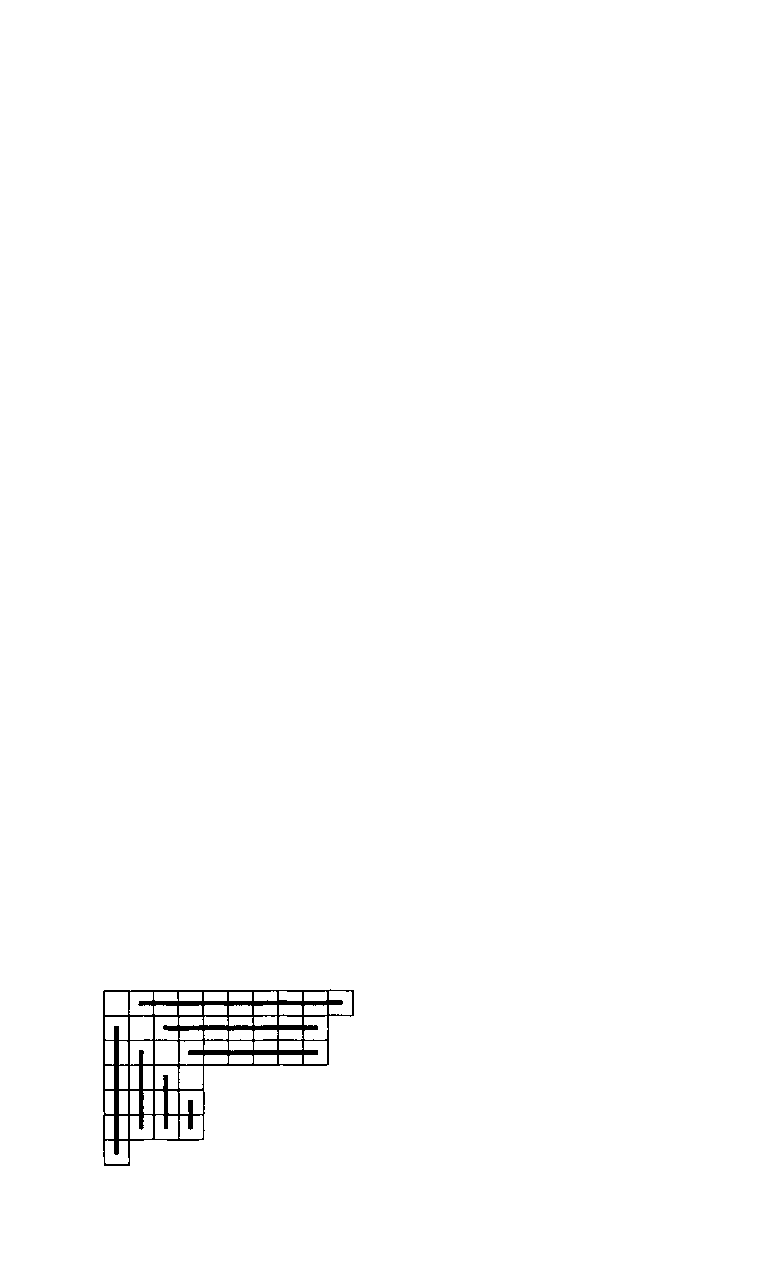
\includegraphics[width=10em]{../figures/FH-pag-51.pdf} &\hspace{-0pt}\raisebox{1.2cm}{$\begin{matrix*}[l]\l=(10,9,9,4,4,4,1)\\\text{Frobenius notation }\begin{pmatrix}9&7&6&0\\2&3&4&5\end{pmatrix}\\\text{modified Frobenius notation }\begin{pmatrix}9.5&7.5&6.5&0.5\\2.5&3.5&4.5&5.5\end{pmatrix}\end{matrix*}$}\end{matrix}\]
\vspace{-1.5em}

\begin{lemma}[Frobenius formula for $C_{(2)}$]
	\vspace{-6pt}
	\deq{\c^\l(C_{(2)})=\frac{\dim\l}{d(d-1)}\sum_{i=1}^r(a_i(a_i+1)-b_i(b_i+1))=\frac{\dim\l}{d(d-1)}\sum_{i=1}^r((a'_i)^2-(b'_i)^2)}
\end{lemma}

\end{frame}

\begin{frame}

From Frobenius formula and $|C_{(2)}|=\begin{pmatrix}d\\2\end{pmatrix}$ it follows that 
\deq{f_2(\l)=\frac{|C_{(2)}|}{\dim \l}\c^\l(C_{(2)})=\frac12\sum_{i=1}^r((a'_i)^2-(b'_i)^2)}

Draw the Young diagram of $\l$ rotated by $135^\circ$ over the real line with opposite orientation as in the picture. 

\[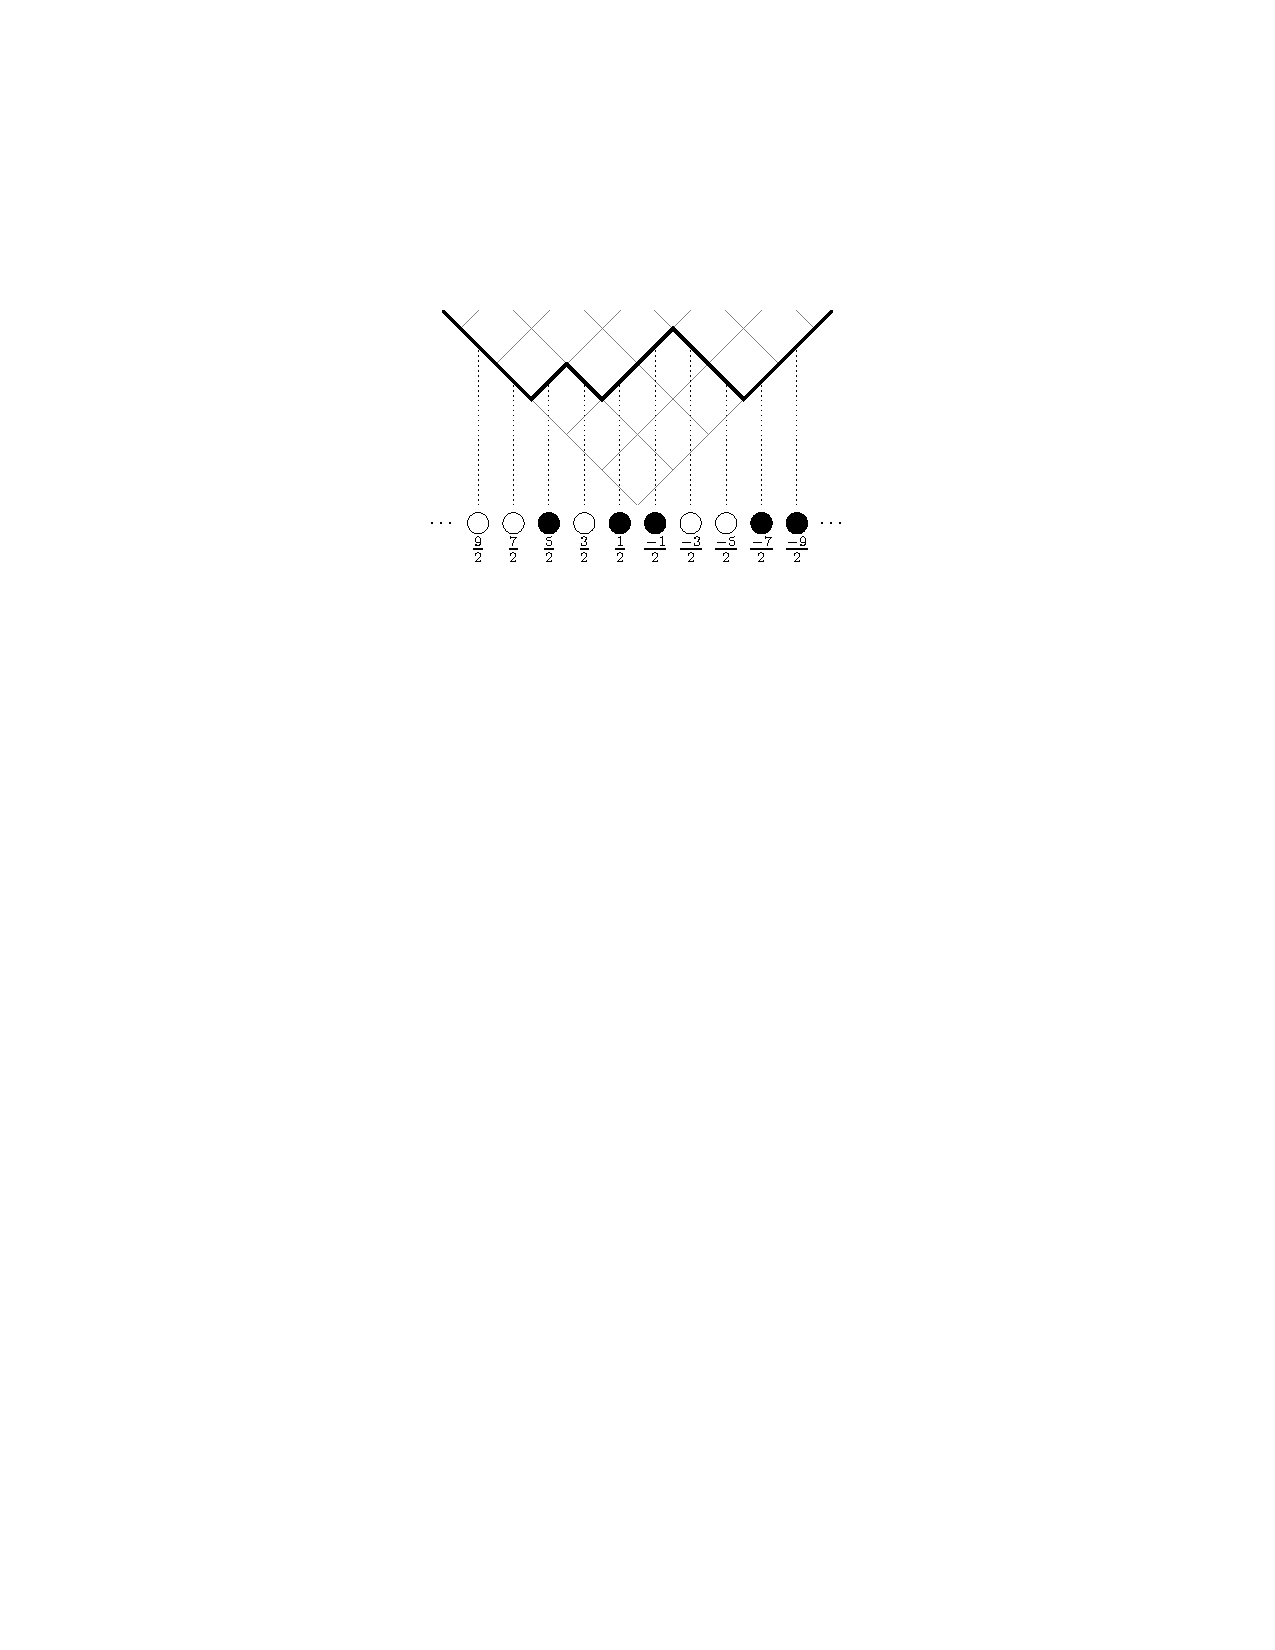
\includegraphics[]{../figures/J-fig-1.pdf}\]

\end{frame}

\begin{frame}

Suppose that $\l$ is made of $k=\ell(\l)$ cycles of lengths $\{\l_1,\ldots,\l_k\}$ where $\l_1\geq\l_2\geq\ldots$. Now consider the ordered set $\{\ti\l_i\}_{i\in\Z_{\geq0}}=\{\l_1,\ldots,\l_k,0,0,\ldots\}$ ending with infinitely many zeros. Then it is clear that black stones are placed in correspondence to elements of 
\deq{\fS_\bullet(\l):=\{\ti\l_i-i+1/2\}\subset\Z+\frac12}
and white stones in correspondence to elements of $\fS_\circ(\l):=(\Z+\frac12)\setminus\fS_\bullet(\l)$. Moreover, the coefficients in the modified Frobenius notation are given by
\deq{\{a'_i\}&=\fS_\bullet^+(\l):=\fS_\bullet\cap(\Z_{\geq0}+1/2)\\
	\{b'_i\}&=\fS_\circ^-(\l):=\fS_\circ\cap(\Z_{\leq0}-1/2)=(\Z_{\leq0}-1/2)\setminus\fS_\bullet(\l)}
Hence we obtained
\deq{f_2(\l)=\sum_{k\in\fS_\bullet^+}\frac{k^2}2-\sum_{k\in\fS_\circ^-}\frac{k^2}2}
Notice also that
\deq{|\l|=\l_1+\cdots+\l_k=a_1'+\cdots+a_k'+b_1'+\cdots+b_k'=\sum_{k\in\fS_\bullet^+} k-\sum_{k\in\fS_\circ^-}k}

\end{frame}

\subsection{Half infinite wedge formalism}

\begin{frame}

\begin{definition}

Let $V$ be a vector space with basis $\{\und k\}$, $k\in\Z+\frac12$. We define the vector space $\hiw$ to be spanned by vectors
\deq{v_S:=\und{s_1}\V\und{s_2}\V\und{s_3}\V\ldots}
where $S=\{s_1>s_2>\dots\}\subset\Z+\frac12$ is a subset \st both
\deq{S^+=S\setminus\Big(\Z_{\leq0}-\frac12\Big)\tand S^-=\Big(\Z_{\leq0}-\frac12\Big)\setminus S}
are finite. We equip $\hiw$ with the inner product $(-,-)$ in which the basis $\{v_S\}$ (for all possible choices of $S$) is orthonormal. 

\end{definition}

For our purposes $S$ is identified with $\fS_\bullet(\l)$ defined before, we denote by $v_\l$ the vector in $\hiw$ corresponding to $S=\fS_\bullet(\l)$. In this case $S^+=\fS_\bullet^+$ and $S^-=\fS_\circ^-$, and finiteness condition simply corresponds to the fact that we have finitely many black stones on the left of the origin and finitely many white stones on the right or the origin, which is automatic for $\fS_\bullet(\l)$. 

\end{frame}

\begin{frame}

\begin{definition}

For all $k\in\Z+\frac12$ define the operators $\p_k$ and $\p_k^*$ on $\hiw$ by 
\deq{\p_k(v):=\und k\V v\tand (v',\p^*_kv)=(\p_kv',v)}
where $v,v'\in\hiw$.
\end{definition}

From the definitions we have
\deq{\p_j\p_k^*+\p_k^*\p_j=\d_{jk}
	\tand
	\p_j\p_k+\p_k\p_j=\p_j^*\p_k^*+\p_k^*\p_j^*=0}
which are known as \emph{fermionic commutation relations}. 

These operators are related to the usual creation and annihilation operators for the \emph{Fermi sea}, by identifying black stones with electrons and white stones with empty energy levels (but in physical literature $\p_k$ and $\p_k^*$ are exchanged). 

Finiteness condition amounts to considering state which are finite energy excitation of the vacuum state. We identify the vacuum of the Fermi sea with the vector $\vac:=\und{-\frac12}\V\und{-\frac32}\V\und{-\frac52}\V\ldots$, where all stones are black (resp. white) on the right (resp. left) of the origin.

All vectors in $\hiw$ can be obtained from $\vac$ by applying $\p_k$ and $\p_k^*$ a finite number of times: $\vac$ is cyclic. 

\end{frame}

\begin{frame}

\begin{definition}

Introduce the \emph{normal ordered product}
\deq{\no{\p_j\p_k^*}\ \ :=\begin{cases}\p_j\p_k^*\quad&k>0\\-\p_k^*\p_j\quad&k<0\end{cases}}

\end{definition}

For $k>0$ (resp. $k<0$), $\no{\p_k\p_k^*}$ gives 1 if we have a black (resp. white) stone in $k$ and zero otherwise.\\
For $j\neq k$ the normal ordered product is the ordinary product due to the fermionic commutation relation $\no{\p_j\p_k^*}\ =\p_j\p_k^*=-\p_k^*\p_j$.\\
The effect of $\no{\p_j\p_k^*}\ $ for $j\neq k$ is to take the black stone in $k$ and move it to the position $j$, unless there is no black stone in $k$ or the position $j$ is already occupied: in such cases it gives the zero vector. \\
Finiteness condition ensures that any operator of the form $\sum_{j,k}a_{jk}\no{\p_j\p_k^*}$ is well defined for any choice of the coefficients $a_{j,k}$. \\
The assignement $E_{jk}\mapsto\ \no{\p_j\p_k^*}$ can be understood as a projective representation of $\fgl(V)$ on $\hiw$. 

\end{frame}

\begin{frame}

\begin{definition}
\vspace{-5pt}
\deq{\cF_2=\sum_{k\in\Z+\frac12}\frac{k^2}2\no{\p_k\p_k^*}}
\end{definition}

It satisfies\\[-15pt]
\deq{\cF_2v_\l=f_2(\l)v_\l}

\begin{definition}
We define the following operators, called \emph{energy operator} and \emph{charge operator} respectively\\[-15pt]
\deq{H:=\sum_{k\in\Z+1/2}k\no{\p_k\p_k^*}
	\qquad
	C:=\sum_{k\in\Z+1/2}\no{\p_k\p_k^*}}
\end{definition}

The physical interpretation of these operators is obvious when we regard a black stone at position $k>0$ as an electron of energy $k$ and charge $+1$ and a white stone at position $k<0$ as a positron of energy $-k$ and charge $-1$. 

We have\\[-15pt]
\deq{Hv_\l=|\l|v_\l}

\end{frame}

\begin{frame}

For the charge operator we have 
\deq{Cv_S=(|S^+|-|S^-|)v_s}
Suppose $Cv_S=c\,v_S$, then $|S^+|=|S^-|+c$. Pick $k\in S$, $k<\min (S^-)$, this means that the stone at $k$ and all those on its right are black. Then $|S^+|=|S^-|+c$ implies that $k=s_{-(k-1/2)+c}$. Hence
\deq{c=\lim_{i\to+\infty}\Big(s_i+i-\frac12\Big)}
In particular, all vectors corresponding to Young diagrams ($S=\fS_\bullet(\l)$) have zero charge. Conversely, any vector of zero charge can be obtained from a Young diagram by taking the partition $\l_i=s_i+i-\frac12$ (omitting the infinitely many $\l_i$ which vanish). We denote by $\hiwz$ the subspace of $\hiw$ of zero charge. From this we get that\\[-15pt]
\deq{\{v_\l\,\big|\,\l\prt d\}}
is a basis for the subspace of $\hiwz$ of energy $d$. Considering all positive values of $d$ we get a basis of the whole charge zero subspace $\hiwz$. 

\end{frame}

\begin{frame}

\begin{definition}
For $n\in\Z_{\neq0}$ define\\[-18pt]
\deq{\a_n:=\sum_{k\in\Z+\frac12}\no{\p_{k-n}\p^*_k}}
\end{definition}

It satisfy $\a_n\und k=\und{k-n}$ and the \emph{Heisenberg commutation relations}
\deq{[\a_n,\a_m]=n\d_{n+m,0}}
From the definition it follows that $\a_n$ and $\a_{-n}$ are adjoint for every $n\in\Z_{\neq0}$.

The effect of this operator in a certain configuration of stones (or electrons) is the following. Pick one and move it to the right by $n$ positions. If the new position is a white stone, make it black and replace the initial black stone by a white one. If the new position is occupied by a black stone, then the operator gives the zero vector (Pauli principle). Then repeat this for all black stones and sum all the resulting vectors to give the final state. Finiteness condition ensures that this operation is well defined. 

\end{frame}

\begin{frame}

\begin{definition}
For any partition $\q=\{\q_1,\ldots,\q_{\ell(\q)}\}\prt|\q|$ define
\deq{\a_{\q}:=\prod_{i=1}^{\ell(\q)}\a_{\q_i}
	\tand
	\a_{-\q}:=\prod_{i=1}^{\ell(\q)}\a_{-\q_i}} 
\end{definition}

The Heisenberg commutation relation ensures that the ordering of the multiplied operators is not relevant and also that $\a_\q$ and $\a_{-\q}$ are adjoint. Note also that $\a_{\q}$ (resp. $\a_{-\q}$) decreases (resp. increases) the energy of states by $|\q|$. Moreover, it is possible to prove that 
\deq{\{\a_{-\q}\vac\,\big|\,\q\prt d\}}
is a basis for the subspace of $\hiwz$ of energy $d$, orthogonal \wrt the inner product $(-,-)$.

\end{frame}

\begin{frame}

The two bases of $\hiwz$ can be related as follows. Let $\l$ be any partition and $n\in\Z_{>0}$. Then graphically we can see that 
\deq{\a_{n}v_\l=\sum_{\l'<\l\atop{\text{$\l/\l'$ skew hook}\atop{|\l/\l'|=n}}}(-1)^{r(\l'/\l)-1}v_{\l'}}
where $r(\l'/\l)$ is the number of rows of $\l'$ touched by $\l'/\l$. 

\[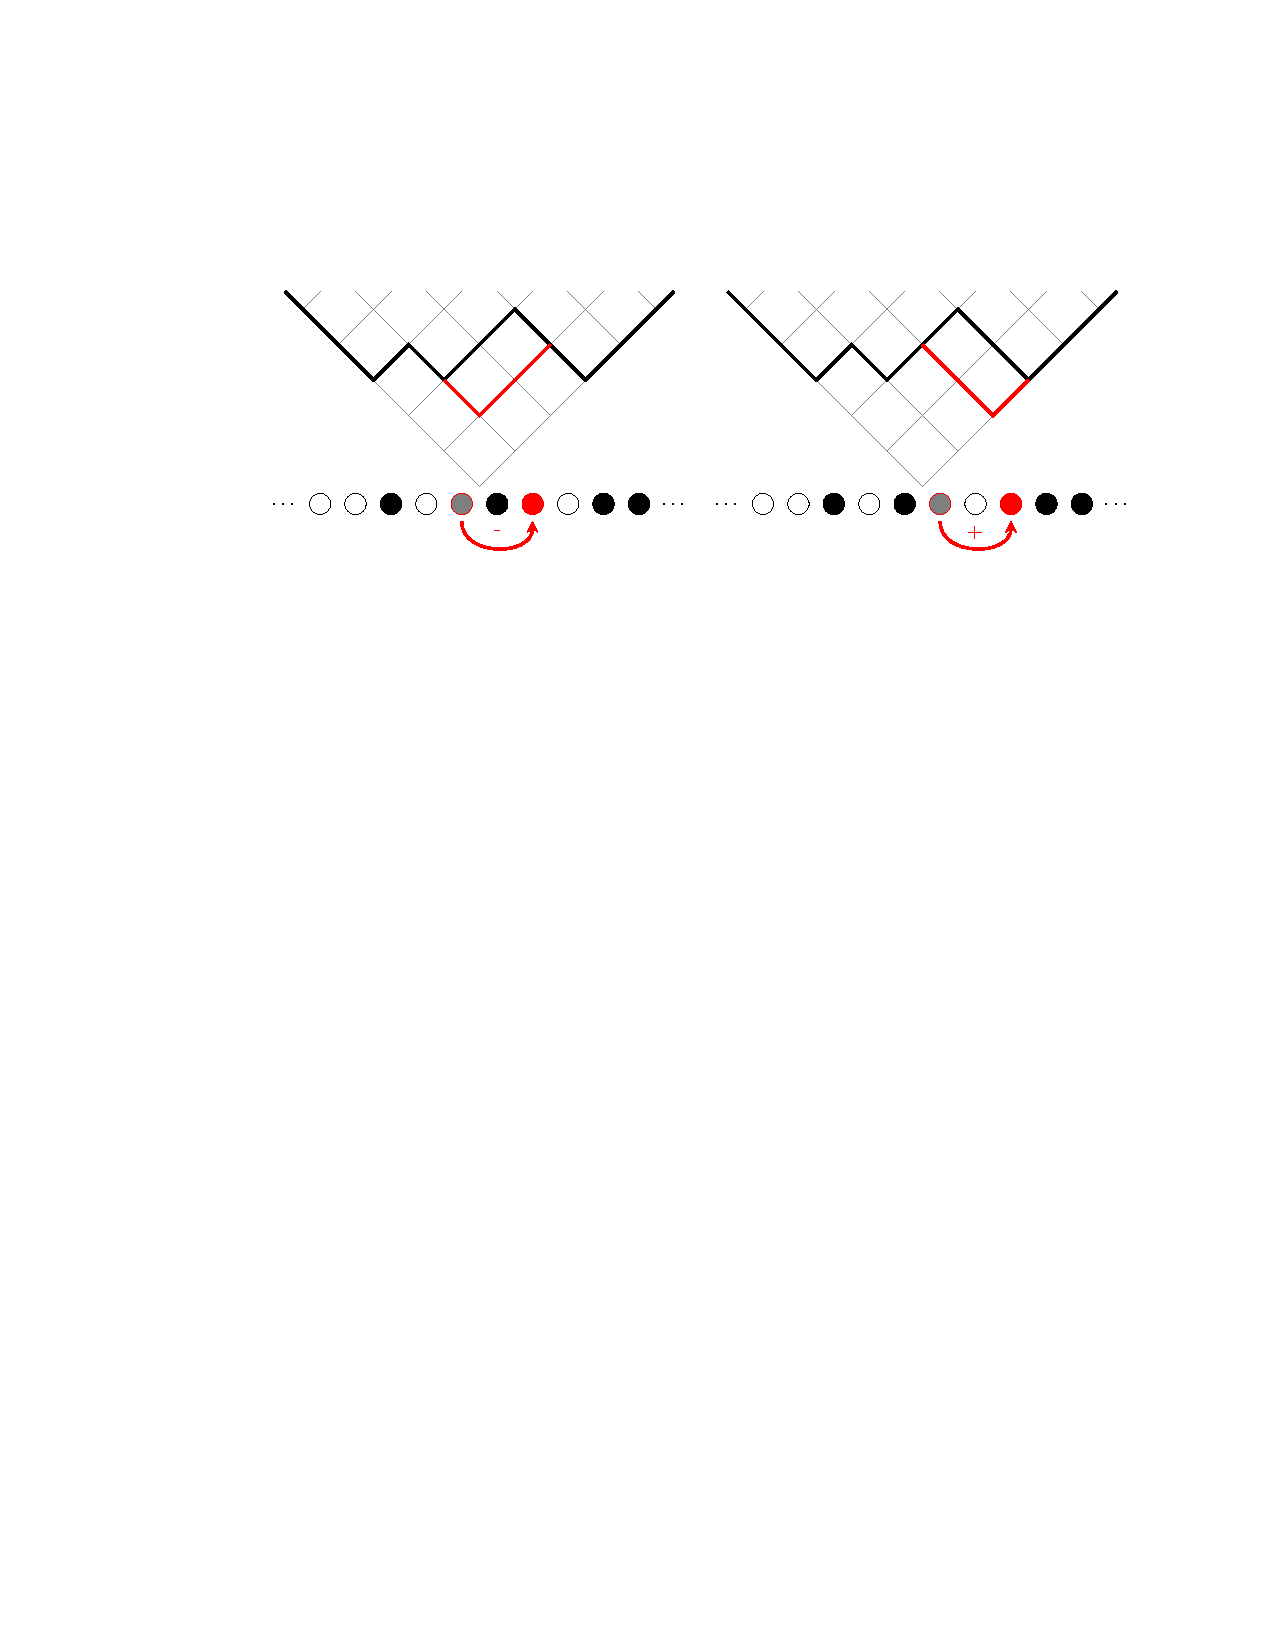
\includegraphics[width=\textwidth]{../figures/J-fig-2.pdf}\]

\end{frame}

\begin{frame}

The two bases of $\hiwz$ can be related as follows. Let $\l$ be any partition and $n\in\Z_{>0}$. Then graphically we can see that 
\deq{\a_{n}v_\l=\sum_{\l'<\l\atop{\text{$\l/\l'$ skew hook}\atop{|\l/\l'|=n}}}(-1)^{r(\l'/\l)-1}v_{\l'}}
where $r(\l'/\l)$ is the number of rows of $\l'$ touched by $\l'/\l$. Compare to
\begin{lemma}[\emph{Murnaghan-Nakayama rule}]
	\deq{\c^\l_{\{(n),\q\}}=\sum_{\l'<\l\atop{\text{$\l/\l'$ skew hook}\atop{|\l/\l'|=n}}}(-1)^{r(\l'/\l)-1}\c^{\l'}_\q}
\end{lemma}
Using these identities we get that for any two partitions $\l$ and $\q$ \st $|\l|=|\q|$ 
\deq{\a_{\q} v_\l=\c_\q^\l v_\emptyset}
and taking the adjoint
\deq{\a_{-\q}\vac=\sum_{\l\prt |\q|}\c_\q^\l v_\l}

\end{frame}


\section{Hurwitz numbers in the half infinite wedge space}

\subsection{Hurwitz numbers using correlators}

\begin{frame}

For $\q=\{\q_1,\ldots,\q_{\ell(\q)}\}\prt d$ and $\q'=\{\q'_1,\ldots,\q'_{\ell(\q')}\}\prt d$ we obtain
\deq{\big(\vac,\a_\q \cF_2^b\a_{-\q'}\vac\big)
	&=\sum_{\l\prt d}\c_{\q'}^\l\big(\vac,\a_\q \cF_2^b v_\l\big)
	=\sum_{\l\prt d}f_2(\l)^b\c_{\q'}^\l\big(\vac,\a_\q v_\l\big)\\
	&=\sum_{\l\prt d}\c_\q^\l f_2(\l)^b\c_{\q'}^\l\big(\vac,\vac\big)
	=\sum_{\l\prt d}\c_{\q}^{\l}f_2(\l)^b\c_{\q'}^{\l}}
and then
\deq{H^\bullet_{d,b}(\q,\q')&=\frac1{\fz(\q)\fz(\q')}\sum_{\l\prt d}\c^\l_{\q}f_2(\l)^b\c^\l_{\q'}=\frac1{\fz(\q)\fz(\q')}\big\la\a_\q \cF_2^b\a_{-\q'}\big\ra}
where the \emph{correlator} of the operator $A$ is defined by $\la A\ra:=(v_\emptyset,Av_\emptyset)$. Similarly
\deq{\fh^\bullet_d(\q,\q')&=\frac1{\fz(\q)\fz(\q')}\sum_{\l\prt d}\c^\l_{\q}e^{z f_2(\l)}\c^\l_{\q'}=\frac1{\fz(\q)\fz(\q')}\big\la\a_\q e^{z\cF_2}\a_{-\q'}\big\ra}

\end{frame}

\begin{frame}

To rewrite the Hurwitz potential we should be able to recover the Schur polynomials from the half infinite wedge formalism. 

\begin{definition}
Given a sequence $t=(t_1,t_2,\ldots)$ define
\deq{\G_\pm(t)=\exp\Bigg(\sum_{n=1}^\infty t_n\a_{\pm n}\Bigg)}
\end{definition}

Note that $\G_+(t)$ and $\G_-(t)$ are adjoint. 
\begin{lemma}
	Consider a set of variables $P=(p_1,p_2,\ldots)$ and denote $p^{(k)}=p_1^k+p_2^k+\cdots$. Then\\[-15pt]
	\deq{\G_-\bigg(p^{(1)},\frac{p^{(2)}}2,\frac{p^{(3)}}3,\cdots\bigg)\vac=\sum_\l s_\l(P)v_\l}
	where $\sum_\l$ runs over all possible partitions (of any number).
\end{lemma}

\end{frame}

\begin{frame}
Introduce the following abbreviations
\deq{\G_+:=\G_+\bigg(p^{(1)},\frac{p^{(2)}}2,\frac{p^{(3)}}3,\cdots\bigg)
	\tand
	\G_-:=\G_-\bigg(p'^{(1)},\frac{p'^{(2)}}2,\frac{p'^{(3)}}3,\cdots\bigg)}
where $P=(p_1,p_2,\ldots)$, $P'=(p'_1,p'_2,\ldots)$. 
Using the lemma we have
\deq{&\big(\vac,\G_+q^He^{z \cF_2}\G_-\vac\big)
	=\sum_{\l,\l'}s_\l(P)s_{\l'}(P')\big(v_\l,q^He^{z \cF_2}v_{\l'}\big)\\
	&\qquad=\sum_{\l,\l'}q^{|\l'|}s_\l(P)e^{z f_2(\l')}s_{\l'}(P')\big(v_\l,v_{\l'}\big)
	=\sum_{\l}q^{|\l|}s_\l(P)e^{z f_2(\l)}s_{\l}(P')}
so
\deq{\fH^\bullet(\{p_j,p_j'\},q,z)=\big\la\G_+q^He^{z \cF_2}\G_-\big\ra}

\end{frame}

\begin{frame}

Summarizing, we obtained the following formulas
\deq{H^\bullet_{d,b}(\q,\q')&=\frac1{\fz(\q)\fz(\q')}\big\la\a_\q \cF_2^b\a_{-\q'}\big\ra\\
	\fh^\bullet_d(\q,\q')&=\frac1{\fz(\q)\fz(\q')}\big\la\a_\q e^{z\cF_2}\a_{-\q'}\big\ra\\
	\fH^\bullet(\{p_j,p_j'\},q,z)&=\big\la\G_+q^He^{z \cF_2}\G_-\big\ra}
From this expression it was shown that the Hurwitz potential $\fH^\bullet$ is the $\w$-function for the Toda lattice hierarchy of Ueno and Takasaki, implying (infinitely) many recursive relations on $\fH^\bullet$. More about this in a forthcoming seminar!
\end{frame}

\subsection{Explicit computation of Hurwitz numbers using commutation relations}

\begin{frame}

Introducing other operators it is possible to rewrite the previous correlators in such a way that their explicit computation is much simplified. In order to simplify the notation, denote $E_{ij}=\ \no{\p_j\p_k^*}$\ .

\begin{definition}
	For $r\in\Z$ define\\[-15pt]
	\deq{\cE_r(z):=\sum_{k\in\Z+\frac12}e^{z(k-r/2)}E_{k-r,k}+\frac{\d_{r,0}}{\varsigma(z)}}
	where $\varsigma(z):=e^{z/2}-e^{-z/2}$.
\end{definition}

The exponent $r/2$ in the definition is used in order to have
\deq{\cE_r(z)^*=\cE_{-r}(z)}
The operators $\cE$ satisfy the following commutation relation
\deq{[\cE_a(z),\cE_b(w)]=\varsigma(\det\left[\begin{smallmatrix}a&z\\b&w\end{smallmatrix}\right])\cE_{a+b}(z+w)}
The operators $\cE$ specialize to the standard bosonic operators on $\hiw$
\deq{\a_k=\cE_k(0)\tcomma k\neq0}

\end{frame}

\begin{frame}

Let's explain the meaning of the additional term arising when $r=0$. We would like to have an operator which acts as
\deq{\und k\mapsto e^{zk}\und{k}}
and the natural candidate is 
\deq{\sum_{k\in\Z+\frac12}e^{zk}\p_{k}\p_k^*}
However applying it to the vacuum the second definition gives for $\Re z>0$
\deq{\sum_{k\in\Z_{\leq0}-\frac12}e^{zk}=e^{-z/2}\sum_{k\in\Z_{\leq0}}e^{zk}=\frac{e^{-z/2}}{1-e^{-z}}=\frac1{\varsigma(z)}}
and diverges for $\Re z=0$. So we regularize
\deq{\sum_{k\in\Z+\frac12}e^{zk}\p_{k}\p_k^*=\sum_{k\in\Z+\frac12}e^{zk}E_{k,k}+\sum_{k\in\Z_{\leq0}-\frac12}e^{zk} \quad\mapsto\quad \sum_{k\in\Z+\frac12}e^{zk}E_{k,k}+\frac1{\varsigma(z)}}
For $r\neq0$ we don't have any problem since $E_{k-r,k}=\p_{k-r}\p_k^*$.

\end{frame}

\begin{frame}

\begin{definition}
	For $k\in\Z_{>0}$ (re)define operators $\cF_k$ and $\cP_k$ by
	\deq{\cF_k=\frac{\cP_k}{k!}=[z^k]\cE_0(z)}
	where $[z^k]\cE_0(z)$ stands for the coefficient of $z^k$ in $\cE_0(z)$. 
\end{definition}

\begin{lemma}
	For $\l$ partition
	\deq{\cP_k v_\l={\bf p}_k(\l)v_\l}
	where $\l=(\l_1,\ldots,\l_k,0,0,\ldots)$ and
	\deq{{\bf p}_k(\l)&=\sum_{i=1}^\infty\bigg[\Big(\l_i-i+\frac12\Big)^k-\Big(-i+\frac12\Big)^k\bigg]+(1-2^{-k})\z(-k)\\
		&=\sum_{i\in\fS_\bullet^+}{i^k}-\sum_{i\in\fS_\circ^-}{i^k}+(1-2^{-k})\z(-k)}
	where $\z$ is the Riemann zeta function.
\end{lemma}

\end{frame}

\begin{frame}

The meaning of the term $(1-2^{-k})\z(-k)$ is as before, that is we would like to have
\deq{\sum_{i=1}^\infty\Big(\l_i-i+\frac12\Big)^k}
but if we consider the partition $\emptyset$ we get the a divergent contribution.

Since $\z(-2)=0$ we get that the new definition of $\cF_2$ coincides with the previous one.

The last formula we need is 
\begin{lemma}
	For $n\in\Z_{\geq1}$
	\deq{e^{z\cF_2}\a_{-n}e^{-z\cF_2}=\cE_{-n}(nz)}
\end{lemma}

\end{frame}

\begin{frame}

Using $\cF_2\vac=0$ we have
\deq{\fh^\bullet_d(\q,\q')&=\frac1{\fz(\q)\fz(\q')}\big\la\a_\q e^{z\cF_2}\a_{-\q'}\big\ra
	=\frac1{\fz(\q)\fz(\q')}\big\la\prod_{i=1}^{\ell(\q)}\a_{\q_i}\prod_{j=1}^{\ell(\q')}\big(e^{z\cF_2}\a_{-\q'_j}e^{-z\cF_2}\big)\ra\\
	&=\frac1{\fz(\q)\fz(\q')}\big\la\prod_{i=1}^{\ell(\q)}\cE_{\q_i}(0)\prod_{j=1}^{\ell(\q')}\cE_{-\q'_j}(z\q'_j)\big\ra}
Using the commutation relation for the operators $\cE$ it is possible to compute the correlator in the previous formula by moving the operators with negative energy on the right and those of positive energy on the left. Then only operators of zero energy survive, so we get a sum of terms of the form $\vars(m_1z)\vars(m_2z)\cdots\cE_0(n_1z)\cE_0(n_2z)\cdots$ for some positive integers $m_1,m_2,\ldots,n_1,n_2,\ldots$.
Now recall
\deq{
	\cE_0(nz)=\sum_{k\in\Z+\frac12}e^{nzk}E_{k-r,k}+\frac1{\vars(nz)}}  
and $E_{k-r,k}\vac=0$ for all $k,r$. Hence $\la\cE_0(nz)\ra=\inv\vars(nz)$ and we get as final result a sum of terms of the form $\vars(m_1z)\vars(m_2z)\cdots\inv\vars(n_1z)\inv\vars(n_2z)\cdots$.  

\end{frame}

%%%%%%% ------ SLIDE ------ %%%%%%%
\begin{frame}[allowframebreaks]
\frametitle{Bibliography}
	
	\nocite{*}
	\printbibliography


\end{frame}


\end{document}